\section{Background estimation}\label{chap6:Backgrounds}

The background processes affecting the analysis phase space are the same as the ones contributing to the SM Higgs boson measurement described in Sec.~\ref{chap5:backgrounds}. The techniques used for the background estimation are the same as well.

The most relevant difference is the addition of the 2 jets category. The WW and top quark background normalizations are estimated in this category using data driven techniques, similarly to the other jet multiplicity categories.

Given the slightly different WW baseline selection with respect to the SM Higgs boson measurement, also the control regions for the top quark and \dytt backgrounds estimation are different, while the WW background normalization is estimated from data in the three signal regions separately, owing to the different \mti shapes for signal and background.

For the estimation of the top quark background, three control regions enriched in b-jets are defined by selecting events that pass the WW baseline selections and applying a b tagging requirement that depends on the jet category as follows:
\begin{itemize}
\item 0 jets category: at least one b-tagged jet with $20 < \pt < 30$\GeV is required;
\item 1 jet category: exactly one b-tagged jet with \pt above 30\GeV is required;
\item 2 jets category: at least one b-tagged jet with \pt above 30\GeV is required.
\end{itemize}
Distributions of the \mti variable in the 0 jets, 1 jet and 2 jets top quark enriched control regions after applying the data driven estimation are shown in Fig.~\ref{fig:TopCtrl}.

\begin{figure}[!htb]
\centering
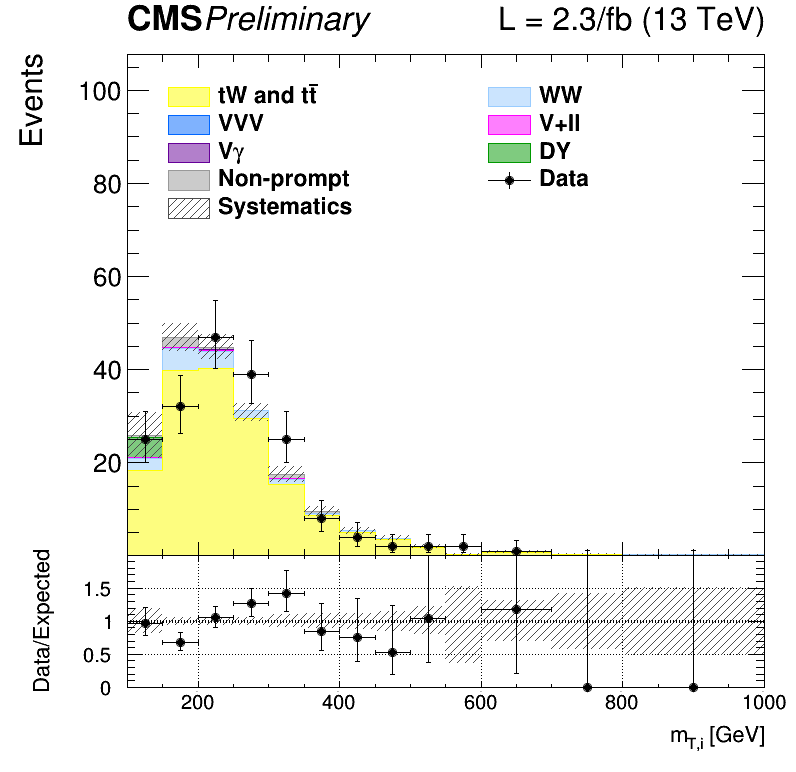
\includegraphics[width=0.45\textwidth]{images/13TeV/HighMass/cratio_hww2l2v_13TeV_top_of0j_mTi.png}
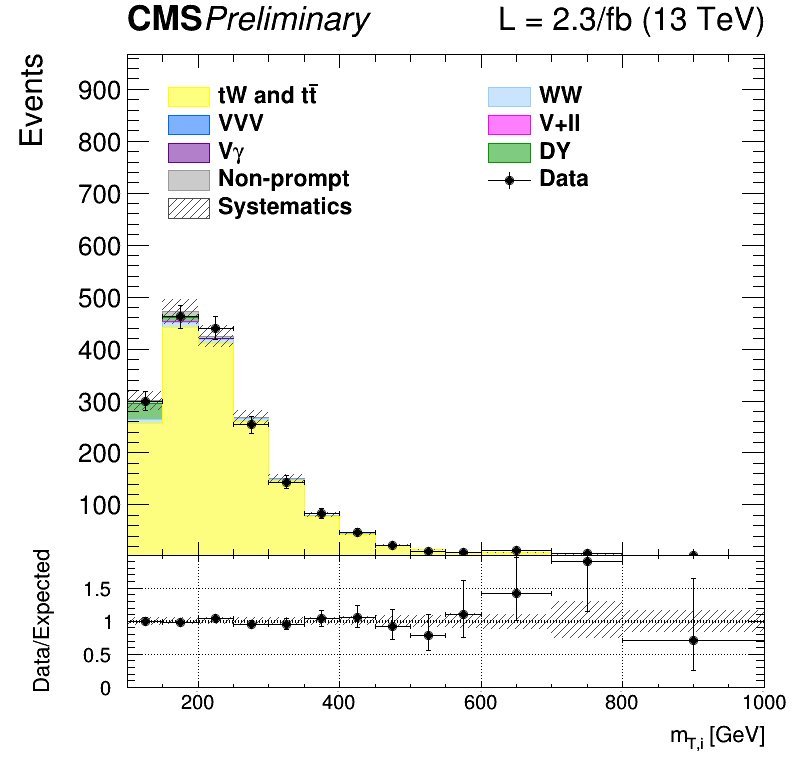
\includegraphics[width=0.45\textwidth]{images/13TeV/HighMass/cratio_hww2l2v_13TeV_top_of1j_mTi.png}
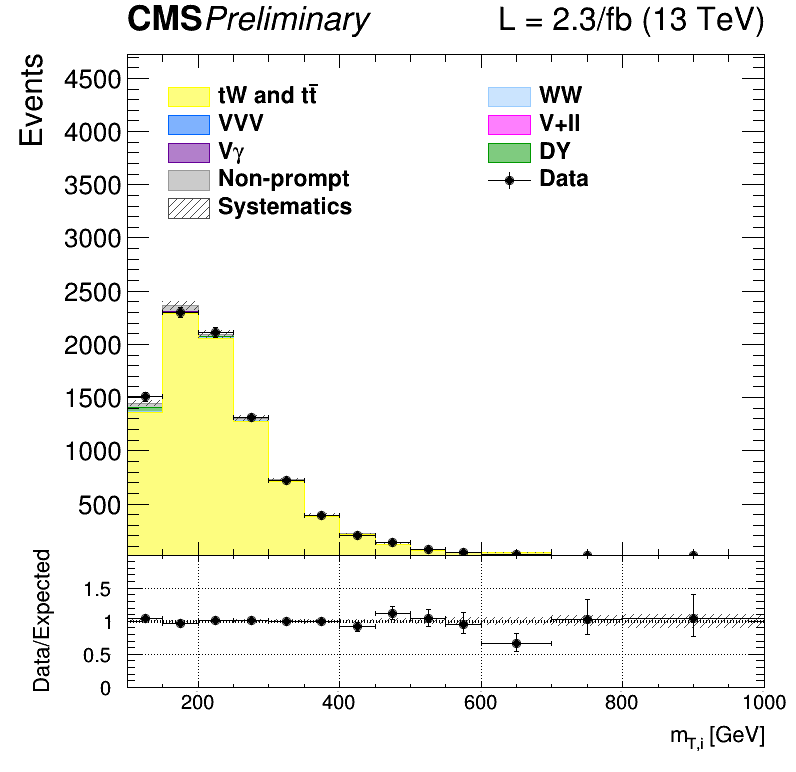
\includegraphics[width=0.45\textwidth]{images/13TeV/HighMass/cratio_hww2l2v_13TeV_top_of2j_mTi.png}
\caption{
Distributions of \mti for events with 0 jets (top left), 1 jet (top right)
and 2 jets (bottom) in top quark enriched control region.
Scale factors estimated from data are not applied. %Data points correspond to the 2015 data set.
}
\label{fig:TopCtrl}
\end{figure}

The jet induced background, here labelled as ``non-prompt'' background so as to highlight that these events do not contain prompt leptons, is estimated using the method described in Sec.~\ref{sec:wjetsbkg}. A cross-check is performed selecting events passing the WW baseline selection but containing an e$\mu$ pair with same charge. The \mti distributions for this phase space are illustrated in Fig.~\ref{fig:13TeV_hm_samesign} for the three jet categories, showing agreement between data and simulation within uncertainties.

\begin{figure}[htb]
\centering
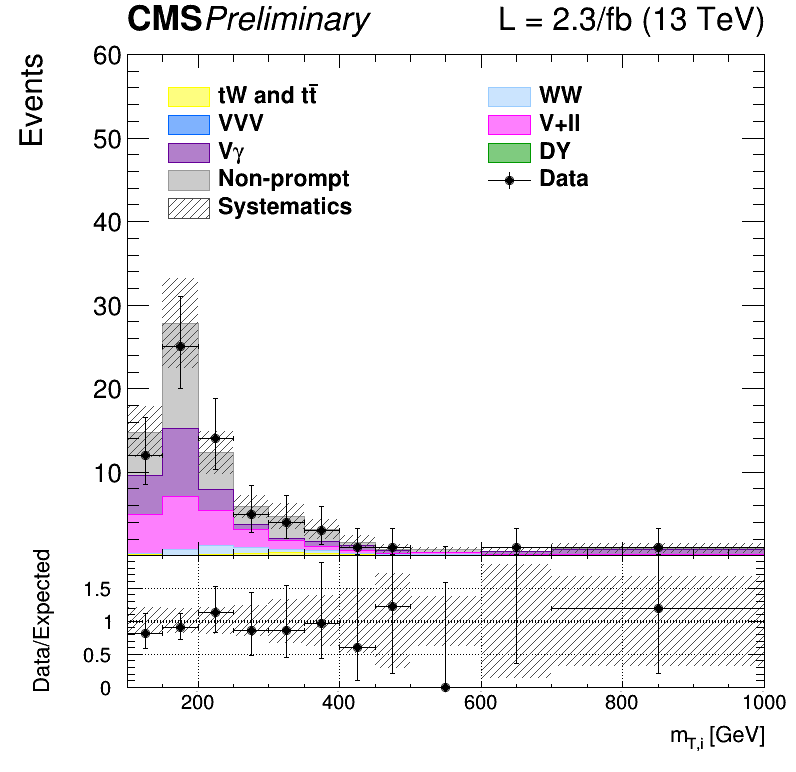
\includegraphics[width=0.45\textwidth]{images/13TeV/HighMass/cratio_hww2l2v_13TeV_ss_of0j_mTi_0j.png}
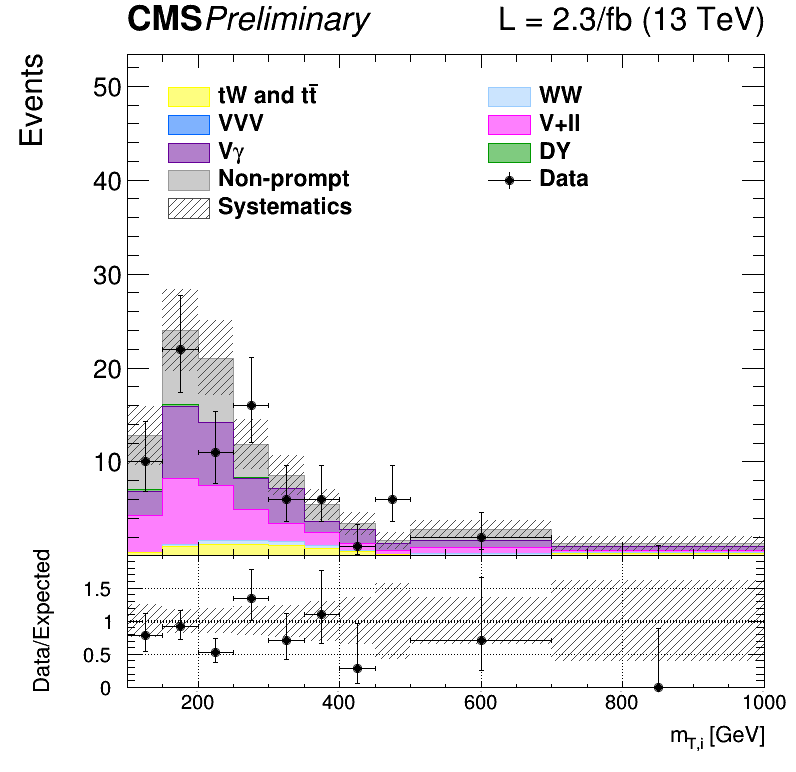
\includegraphics[width=0.45\textwidth]{images/13TeV/HighMass/cratio_hww2l2v_13TeV_ss_of1j_mTi_1j.png}
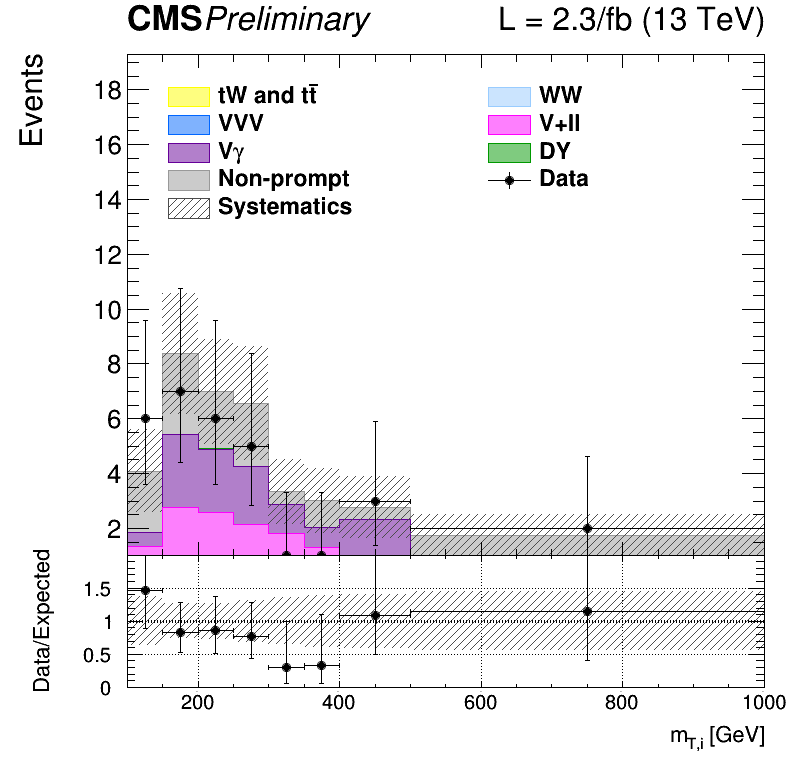
\includegraphics[width=0.45\textwidth]{images/13TeV/HighMass/cratio_hww2l2v_13TeV_ss_of2j_mTi_VBF.png}
\caption{
Distributions of \mti for events with 0 jets (top left), 1 jet (top right) and 2 jets (bottom) in the same-charge dilepton
control region. The last bin of the histograms includes overflows. %Data points correspond to the 2015 data set.
}
\label{fig:13TeV_hm_samesign}
\end{figure}

Due to the selections on the leptons \pt and on \mll in the WW baseline requirements, the contribution of the \dytt background is very small in the signal regions, especially in the VBF phase space. The normalization of this background is estimated from a control region in data, defined in the same way as explained in \ref{chap5:DYbackground}, for the 0 and 1 jets categories. In the VBF category the normalization of this background is taken from simulation.

Other minor background processes are estimated as described in \ref{chap5:otherBackgrounds}.













